% docs/latex/search-process.tex
\documentclass{standalone}
\usepackage{tikz}
\usetikzlibrary{arrows.meta,backgrounds}

\begin{document}
\pagecolor{white}
\color{black}
	\pagecolor{white}
	\color{black}
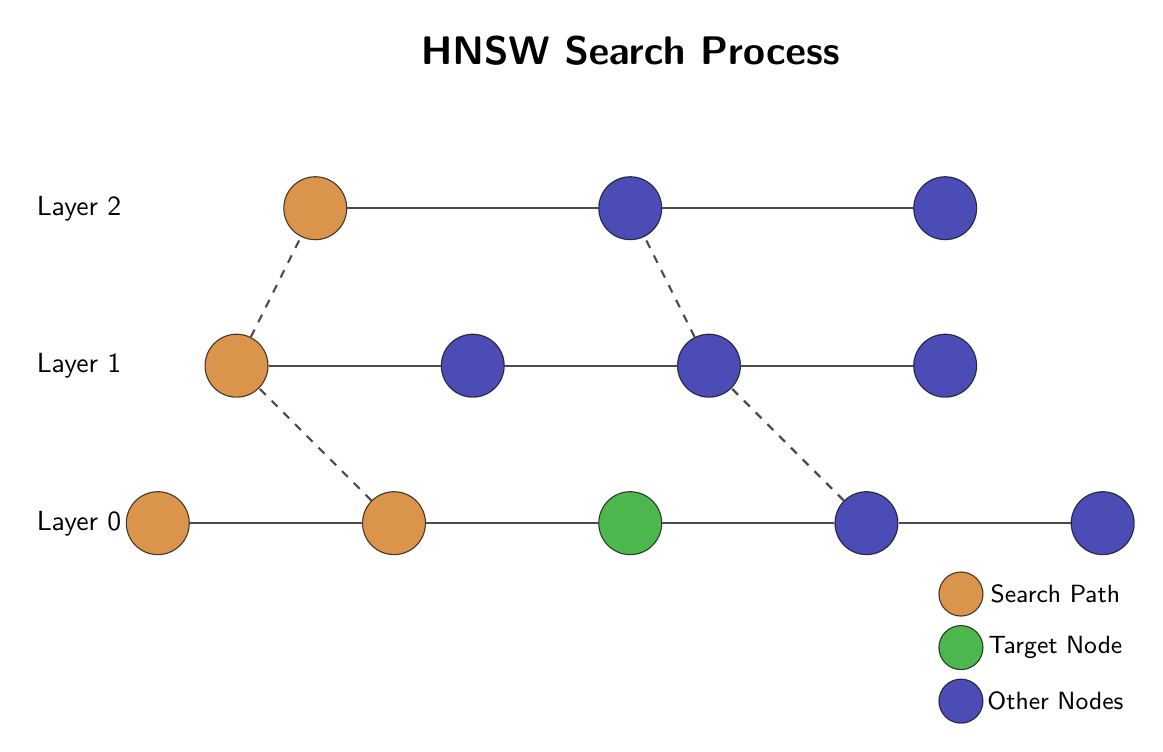
\begin{tikzpicture}[
    node/.style={circle, draw, fill=#1, minimum size=0.8cm, opacity=0.7},
    search node/.style={node=orange!80!black},
    target node/.style={node=green!60!black},
    other node/.style={node=blue!60!black},
    connection/.style={-, thick, gray!60!black},
    vertical connection/.style={connection, dashed}
]

% Title
\node[font=\Large\sffamily\bfseries] at (0,4) {HNSW Search Process};

% Layer labels
\node[font=\sffamily] at (-7,2) {Layer 2};
\node[font=\sffamily] at (-7,0) {Layer 1};
\node[font=\sffamily] at (-7,-2) {Layer 0};

% Layer 2
\begin{scope}[yshift=2cm]
    \node[search node] (L2N1) at (-4,0) {};
    \node[other node] (L2N2) at (0,0) {};
    \node[other node] (L2N3) at (4,0) {};
    \draw[connection] (L2N1) -- (L2N2);
    \draw[connection] (L2N2) -- (L2N3);
\end{scope}

% Layer 1
\begin{scope}
    \node[search node] (L1N1) at (-5,0) {};
    \node[other node] (L1N2) at (-2,0) {};
    \node[other node] (L1N3) at (1,0) {};
    \node[other node] (L1N4) at (4,0) {};
    \draw[connection] (L1N1) -- (L1N2);
    \draw[connection] (L1N2) -- (L1N3);
    \draw[connection] (L1N3) -- (L1N4);
    \draw[vertical connection] (L1N1) -- (L2N1);
    \draw[vertical connection] (L1N3) -- (L2N2);
\end{scope}

% Layer 0
\begin{scope}[yshift=-2cm]
    \node[search node] (L0N1) at (-6,0) {};
    \node[search node] (L0N2) at (-3,0) {};
    \node[target node] (L0N3) at (0,0) {};
    \node[other node] (L0N4) at (3,0) {};
    \node[other node] (L0N5) at (6,0) {};
    \draw[connection] (L0N1) -- (L0N2);
    \draw[connection] (L0N2) -- (L0N3);
    \draw[connection] (L0N3) -- (L0N4);
    \draw[connection] (L0N4) -- (L0N5);
    \draw[vertical connection] (L0N2) -- (L1N1);
    \draw[vertical connection] (L0N4) -- (L1N3);
\end{scope}

% Legend
\begin{scope}[shift={(4.2,-3.9)}]
    \node[search node, scale=0.7] at (0,1) {};
    \node[font=\small\sffamily] at (1.2,1) {Search Path};
    
    \node[target node, scale=0.7] at (0,0.32) {};
    \node[font=\small\sffamily] at (1.2,0.32) {Target Node};
    
    \node[other node, scale=0.7] at (0,-0.36) {};
    \node[font=\small\sffamily] at (1.2,-0.36) {Other Nodes};
\end{scope}

\end{tikzpicture}
\end{document}